\documentclass{article}
\usepackage{amsmath} 
\usepackage{graphicx}
\usepackage{cite}

\graphicspath{{images/}}

\title{Assignment 4}
\author{Kaustubh Titare \\ Roll No: CH22B072 }


\date{\today}
\begin{document}
\maketitle

\begin{center}
    GitHub ID : 0kt1
\end{center}
\title{Heron's Formula}

\maketitle

\section{CH22B072}
\subsection{Introduction}
Heron's formula \footnote{Derived from Heron of Alexandria, a Greek mathematician (c. 10-70 AD).} is used to calculate the area ($A$) of a triangle when the lengths of its sides ($a$, $b$, and $c$) are known. The formula is given as:

\[
A = \sqrt{s(s-a)(s-b)(s-c)}
\]

where $s$ is the semi-perimeter of the triangle, defined as:

\[
s = \frac{a+b+c}{2}
\]
Proof of this formula can be found here\cite{AHistoryOfGreekMatheMaticsVol2} and\cite{heronFormula2009}.

\begin{figure}[ht]
  \centering
  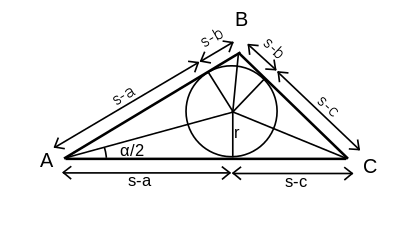
\includegraphics[width=0.6\textwidth]{heron.png}
  \caption{Geometric Significance}
\end{figure}

\subsection{Example Calculation}
Let's consider a triangle with side lengths $a = 5$, $b = 7$, and $c = 8$. We can calculate the area using Heron's formula:

\[
s = \frac{5+7+8}{2} = 10
\]

\[
A = \sqrt{10(10-5)(10-7)(10-8)} = \sqrt{10 \cdot 5 \cdot 3 \cdot 2} = \sqrt{300} \approx 17.32
\]

Therefore, the area of the triangle is approximately 17.32 square units.

\subsection{Conclusion}
Heron's formula provides a convenient method for calculating the area of a triangle using its side lengths. It is widely used in various mathematical and geometric applications.



\bibliographystyle{plain}
\bibliography{refer}

\end{document}

